\documentclass[12pt]{article}

\usepackage{enumitem,stoversymb,graphicx}
\usepackage[letterpaper, margin=0.1in, top=0.75in, bottom=1in,left=0.1in]{geometry}
\usepackage[draft]{pgf}
%\graphicspath{ {../.././parametric/} }

\everymath{\displaystyle}
%\pagenumbering{gobble}

%\usepackage{multicol}
%\usepackage{tcolorbox}
%\usepackage{tikz}

\usepackage{array}
\newcolumntype{L}[1]{>{\raggedright\let\newline\\\arraybackslash\hspace{0pt}}m{#1}}
\newcolumntype{C}[1]{>{\centering\let\newline\\\arraybackslash\hspace{0pt}}m{#1}}
\newcolumntype{R}[1]{>{\raggedleft\let\newline\\\arraybackslash\hspace{0pt}}m{#1}}
\newcolumntype{N}{@{}m{0pt}@{}}

\title{\vspace{-0.75in}\Huge{Curves You Should Know}\vspace{-0.5in}}
\date{}
	
\begin{document}
	\maketitle
	\begin{center}
	\begin{tabular}{|C{2.75in}|C{1.625in}|C{1.625in}|C{1.625in}|N}
	\hline
	\textbf{Graph} & 
	\textbf{Cartesian} & 
	\textbf{Parametric} & 
	\textbf{Polar}& \\[5mm]
	
	\hline
	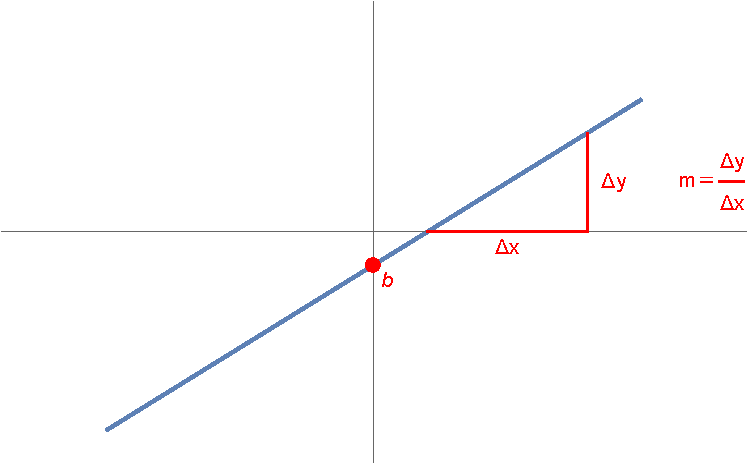
\includegraphics[trim={0 -4.5mm 0 -4.5mm}, clip, height=1.875in]{1_Lines} & 
	$y=mx+b$ & 
	$\begin{array}{c}
	x=at\\
	y=ct+b,\\[6mm]
	\end{array}$ \newline where $ m=\frac{c}{a}$ \vspace{-14mm} & 
	$r(\theta)=\frac{b}{\sin{\theta}-m\cos{\theta}}$ & \\
	
	\hline
	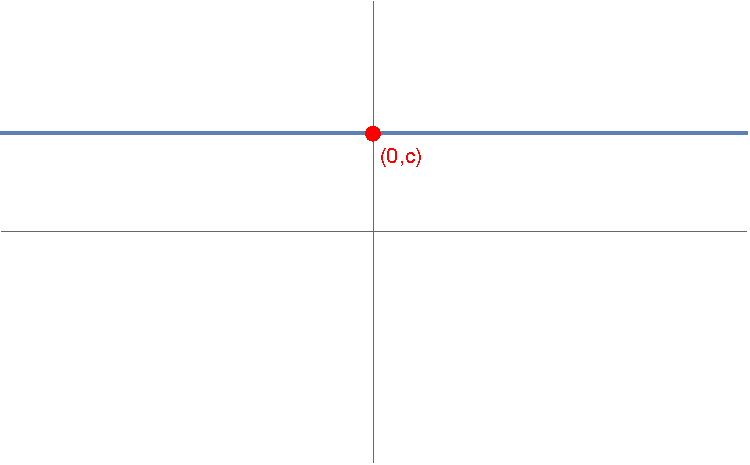
\includegraphics[trim={0 -4.5mm 0 -4.5mm}, clip, height=1.875in]{1_Lines2} & 
	$y=c$ & 
	$\begin{array}{c}
	x=at+b\\
	y=c
	\end{array}$ & 
	$r(\theta)=\frac{c}{\sin{\theta}}$ & \\
	
	\hline
	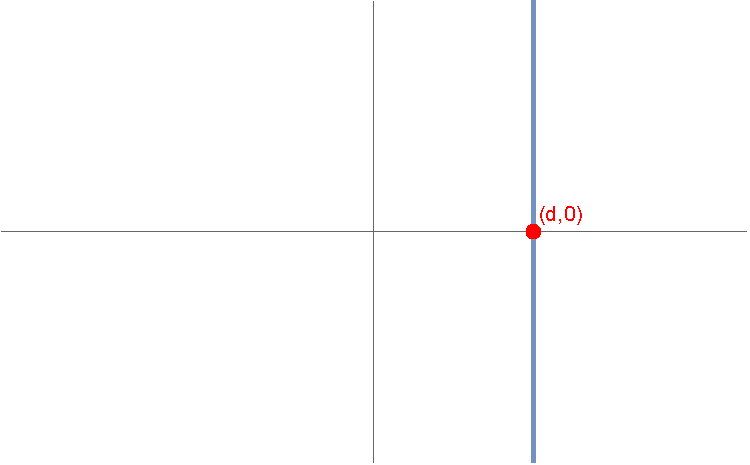
\includegraphics[trim={0 -4.5mm 0 -4.5mm}, clip, height=1.875in]{1_Lines3} &
	$x = d$ &
	$\begin{array}{c}
	x=d\\
	y=at+b
	\end{array}$ &
	$r(\theta) = \frac{d}{\cos{\theta}}$ & \\
	
	\hline
	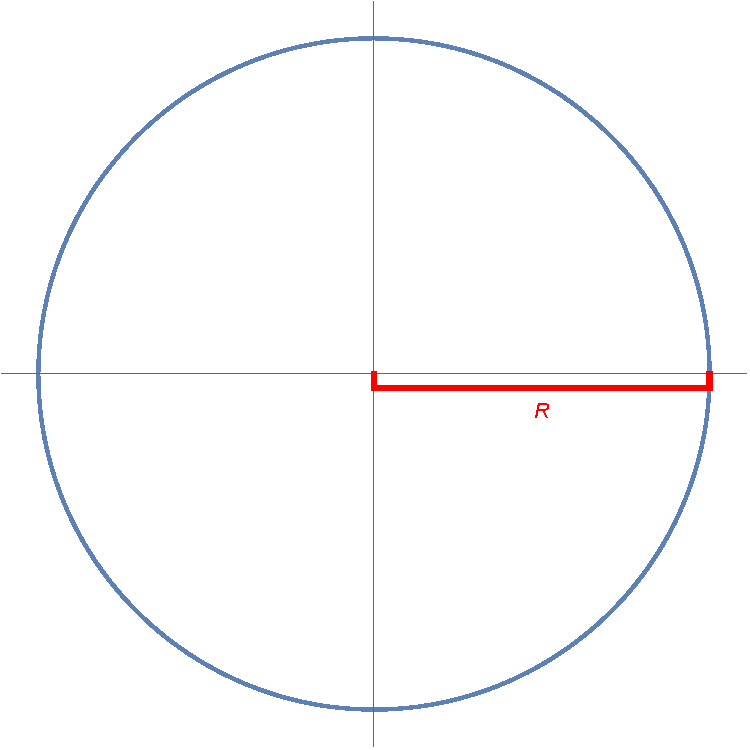
\includegraphics[trim={0 -4.5mm 0 -4.5mm}, clip, height=1.875in]{2_Circles}  &
	$x^2+y^2=R^2$ &
	$\begin{array}{c}
	x=R\cos{t}\\
	y=R\sin{t},\\[6mm]
	\end{array}$ $0\leq t\leq 2\pi$ \vspace{-10mm}& 
	$r(\theta)=R$ & \\
	
	\hline
	\end{tabular}
	\end{center}

	\newpage
	
	\begin{center}
	\begin{tabular}{|C{2.75in}|C{1.625in}|C{1.625in}|C{1.625in}|N}
		\hline
		\textbf{Graph} & 
		\textbf{Cartesian} & 
		\textbf{Parametric} & 
		\textbf{Polar}& \\[5mm]
		
		\hline
		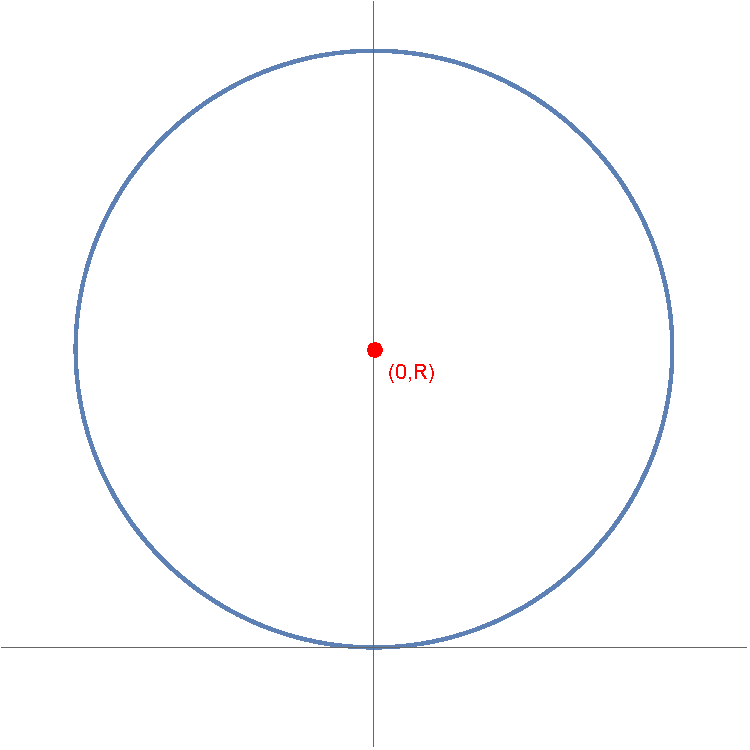
\includegraphics[trim={0 0 0 -4.5mm}, clip, height=1.875in]{2_Circles2} \newline ($R<0$ flips across $x$-axis) \vspace{3mm} &	
		$x^2+(y-R)^2=1$ & 
		$\begin{array}{c}
		x=2R\sin{t}\cos{t}\\
		y=2R\sin{t}\sin{t},\\[6mm]
		\end{array}$ $0\leq t\leq 2\pi$ \vspace{-10mm} & 
		$r(\theta)=2R\sin{\theta}$ & \\
		
		\hline
		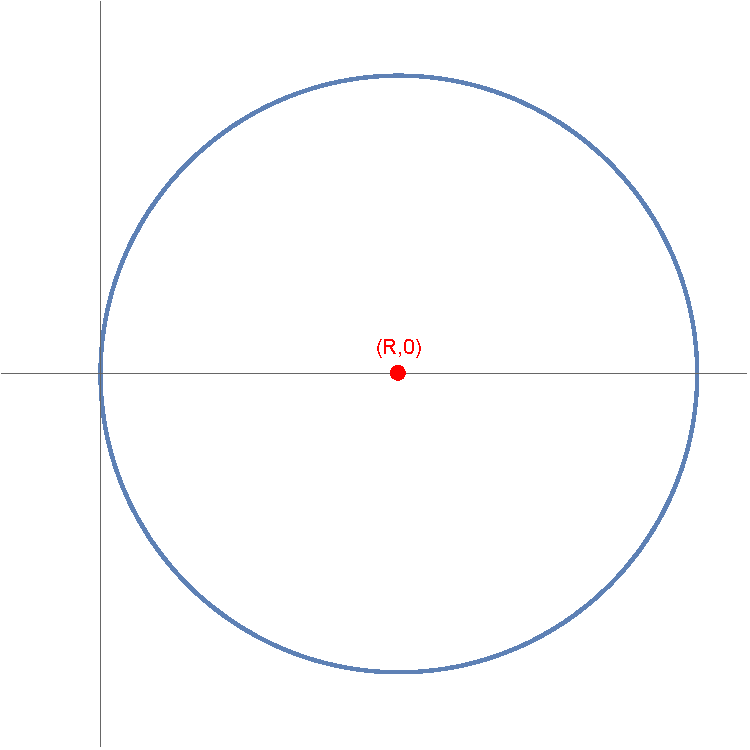
\includegraphics[trim={0 0 0 -4.5mm}, clip, height=1.875in]{2_Circles3} \newline ($R<0$ flips across $y$-axis) \vspace{3mm} &
		$(x-R)^2+y^2=1$ & 
		$\begin{array}{c}
		x=2R\cos{t}\cos{t}\\
		y=2R\cos{t}\sin{t},\\[6mm]
		\end{array}$ $0\leq t\leq 2\pi$ \vspace{-10mm} & 
		$r(\theta)=2R\cos{\theta}$ & \\
		
		\hline
		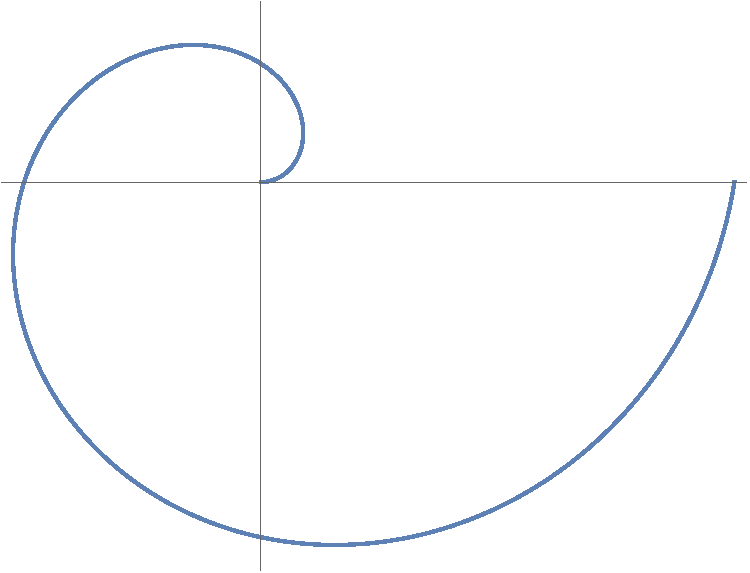
\includegraphics[trim={0 -4.5mm 0 -4.5mm}, clip, height=1.875in]{3_Spiral} \newline ($0\leq t\leq n\pi$ crosses $x$-axis $n$ times) \vspace{3mm} &
		$x^2+y^2=\arctan^2\left(\frac{y}{x}\right)$ & 
		$\begin{array}{c}
		x=t\cos{t}\\
		y=t\sin{t},\\[6mm]
		\end{array}$ $0\leq t\leq 2\pi$ \vspace{-10mm} & 
		$r(\theta)=\theta$ & \\
		
		\hline
		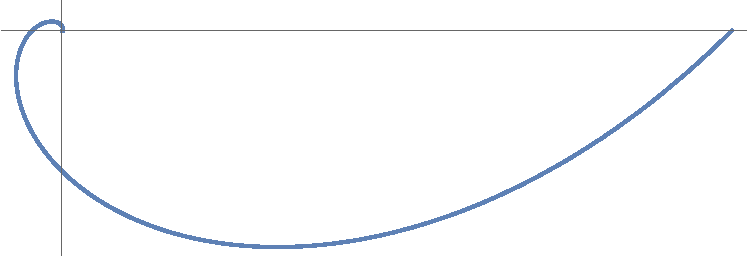
\includegraphics[trim={0 -14mm 0 -14mm}, clip, width=2.75in]{3_Spiral2} \newline ($0\leq t\leq n\pi$ crosses $x$-axis $n$ times) \vspace{3mm} &
		$x^2+y^2=e^{2\arctan\left(\frac{y}{x}\right)}$ & 
		$\begin{array}{c}
		x=e^t\cos{t}\\
		y=e^t\sin{t},\\[6mm]
		\end{array}$ $0\leq t\leq 2\pi$ \vspace{-10mm} & 
		$r(\theta)=e^\theta$ & \\
		
		\hline
	\end{tabular}
	\end{center}

	\begin{center}
	\begin{tabular}{|C{2.75in}|C{1.625in}|C{1.625in}|C{1.625in}|N}
		\hline
		\textbf{Graph} & 
		\textbf{Cartesian} & 
		\textbf{Parametric} & 
		\textbf{Polar}& \\[5mm]
		
%		\hline
%		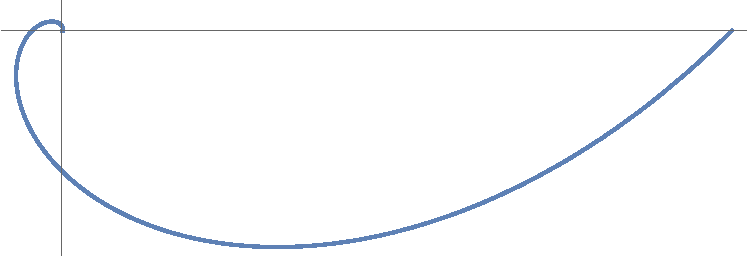
\includegraphics[trim={0 -14mm 0 -14mm}, clip, width=2.75in]{3_Spiral2} \newline ($0\leq t\leq n\pi$ crosses $x$-axis $n$ times) \vspace{3mm} &
%		Cycloid & 
%		$\begin{array}{c}
%		x=r(t-\sin{t})\\
%		y=r(1-\cos{t}),\\[6mm]
%		\end{array}$ $0\leq t\leq 2\pi$ \vspace{-10mm} & 
%		--- & \\

		\hline
		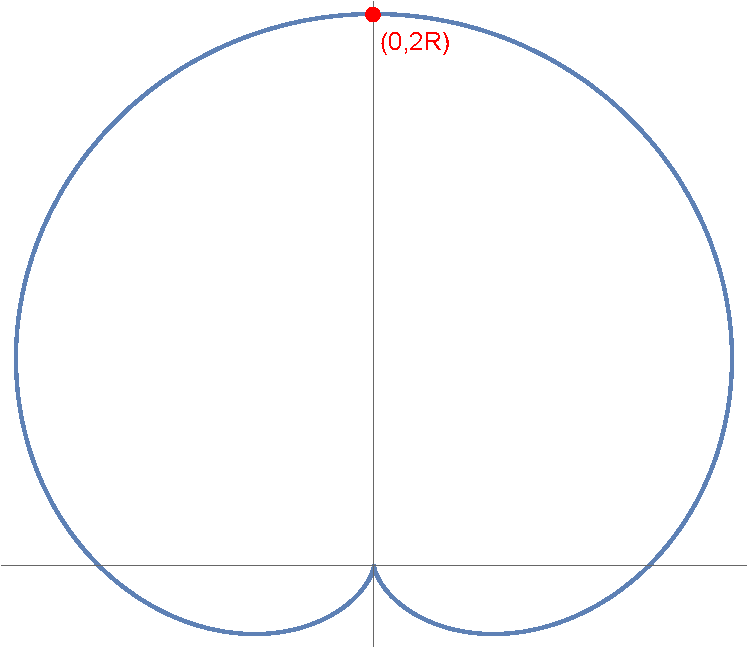
\includegraphics[trim={0 -4.5mm 0 -4.5mm}, clip, height=1.8in]{4_Cardioid} \newline \scriptsize{($R<0$ flips across $x$-axis)} \vspace{3mm} &
		--- & 
		$\begin{array}{c}
		x=R(1+\sin{t})\cos{t}\\
		y=R(1+\sin{t})\sin{t},\\[6mm]
		\end{array}$ $0\leq t\leq 2\pi$ \vspace{-10mm} & 
		$r(\theta)=R(1+\sin{\theta})$ & \\
		
		\hline
		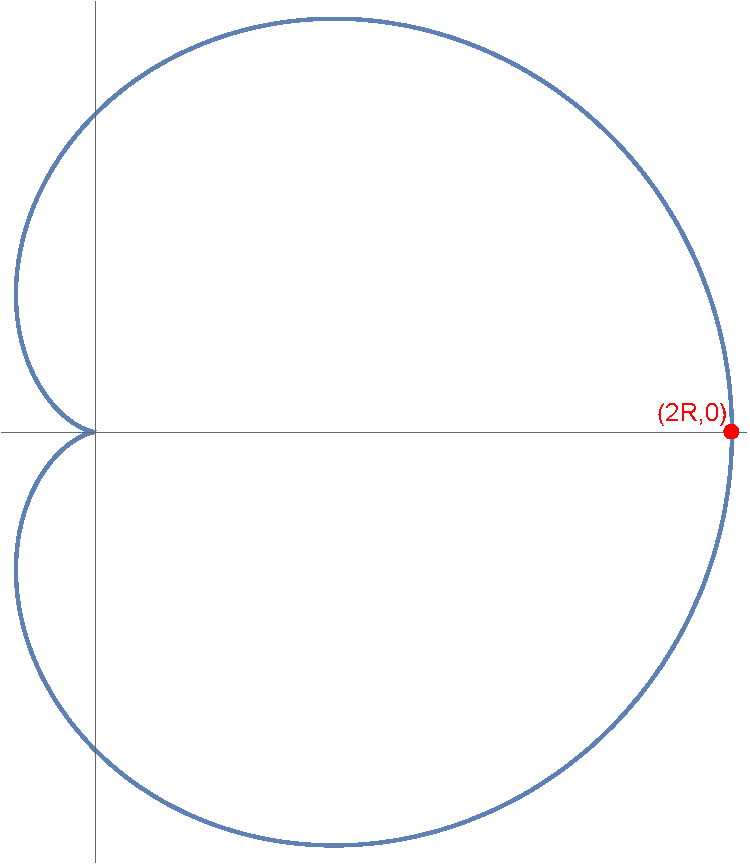
\includegraphics[trim={0 -4.5mm 0 -4.5mm}, clip, height=1.8in]{4_Cardioid2} \newline \scriptsize{($R<0$ flips across $y$-axis)} \vspace{3mm} &
		--- & 
		$\begin{array}{c}
		x=R(1+\cos{t})\cos{t}\\
		y=R(1+\cos{t})\sin{t},\\[6mm]
		\end{array}$ $0\leq t\leq 2\pi$ \vspace{-6mm} & 
		$r(\theta)=R(1+\cos{\theta})$ & \\
		
		\hline
		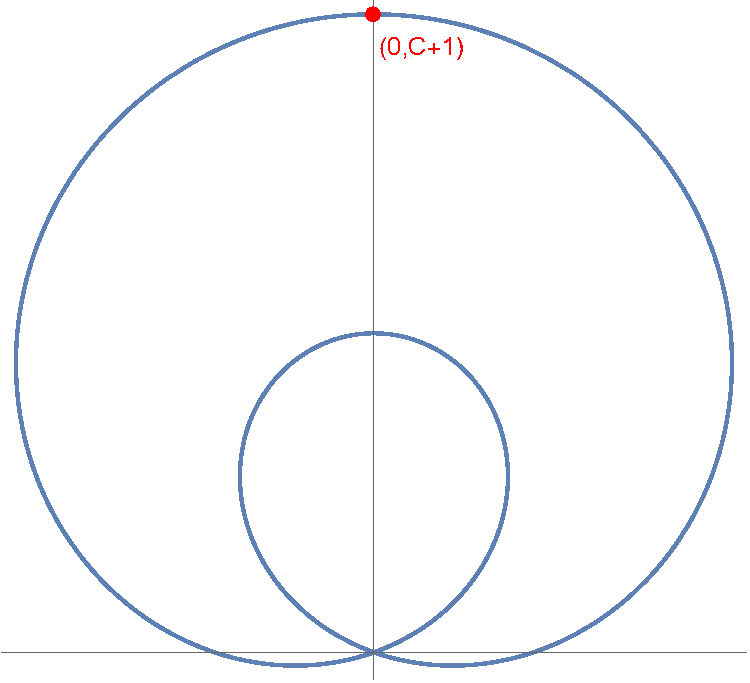
\includegraphics[trim={0 -4.5mm 0 -4.5mm}, clip, height=1.8in]{5_Limacon} \newline \scriptsize{($C<0$ flips across $x$-axis) \newline (Big/small $C$ = big/small inner loop)} \vspace{3mm} &
		--- & 
		$\begin{array}{c}
		x=(1+C\sin{t})\cos{t}\\
		y=(1+C\sin{t})\sin{t},\\[6mm]
		\end{array}$ $0\leq t\leq 2\pi$ \vspace{-10mm} & 
		$r(\theta)=1+C\sin{\theta}$ & \\
		
		\hline
		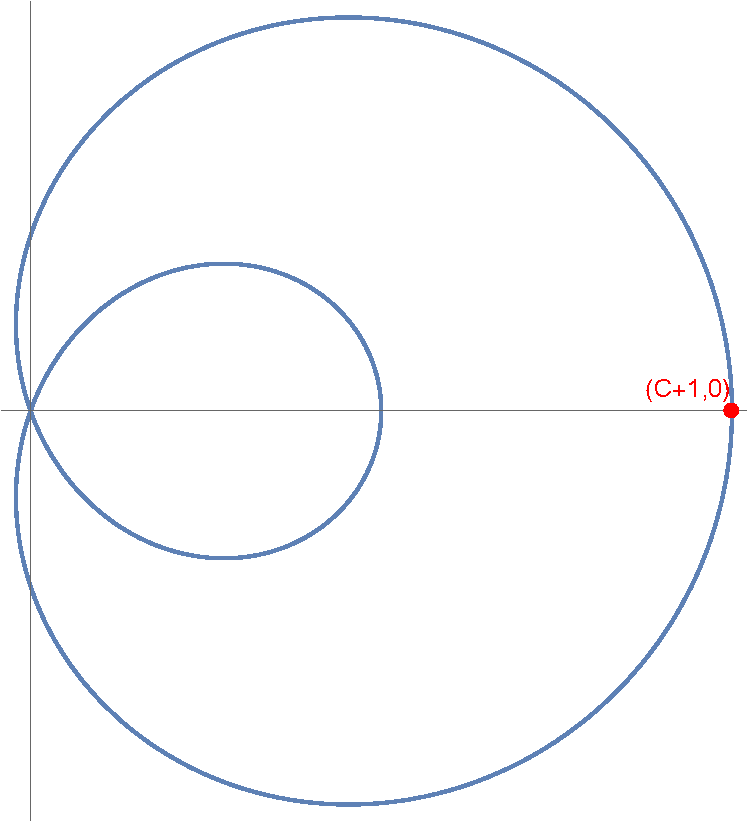
\includegraphics[trim={0 -4.5mm 0 -4.5mm}, clip, height=1.8in]{5_Limacon2} \newline \scriptsize{($C<0$ flips across $y$-axis) \newline (Big/small $C$ = big/small inner loop)} \vspace{3mm} &
		--- & 
		$\begin{array}{c}
		x=(1+C\cos{t})\cos{t}\\
		y=(1+C\cos{t})\sin{t},\\[6mm]
		\end{array}$ $0\leq t\leq 2\pi$ \vspace{-10mm} & 
		$r(\theta)=1+C\cos{\theta}$ & \\
		
		\hline
	\end{tabular}
	\end{center}

	\begin{center}
	\begin{tabular}{|C{2.75in}|C{1.625in}|C{1.625in}|C{1.625in}|N}
		\hline
		\textbf{Graph} & 
		\textbf{Cartesian} & 
		\textbf{Parametric} & 
		\textbf{Polar}& \\[5mm]
		
		\hline
		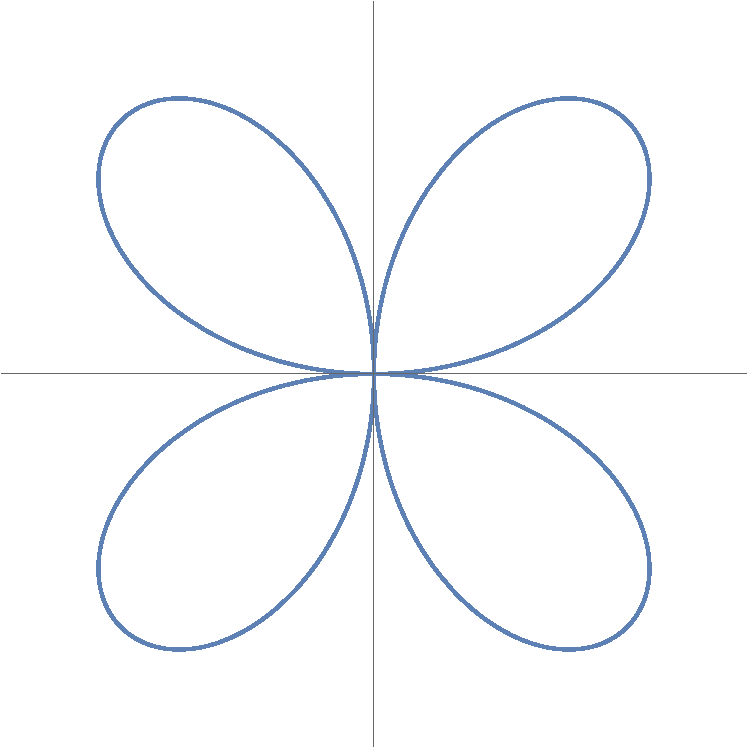
\includegraphics[trim={0 0 0 -4.5mm}, clip, height=1.7in]{6_Rose} \newline \scriptsize{($C<0$ flips across $x$-axis) \newline $2C$ petals} \vspace{3mm} &
		--- & 
		$\begin{array}{c}
		x=\sin({Ct})\cos{t}\\
		y=\sin({Ct})\sin{t},\\[8mm]
		\end{array}$ $0\leq t\leq 2\pi$ \newline $C$ even \vspace{-14mm} & 
		$r(\theta)=\sin(C\theta)$ \newline \vspace{9mm} $C$ even \vspace{-12mm} & \\
		
		\hline
		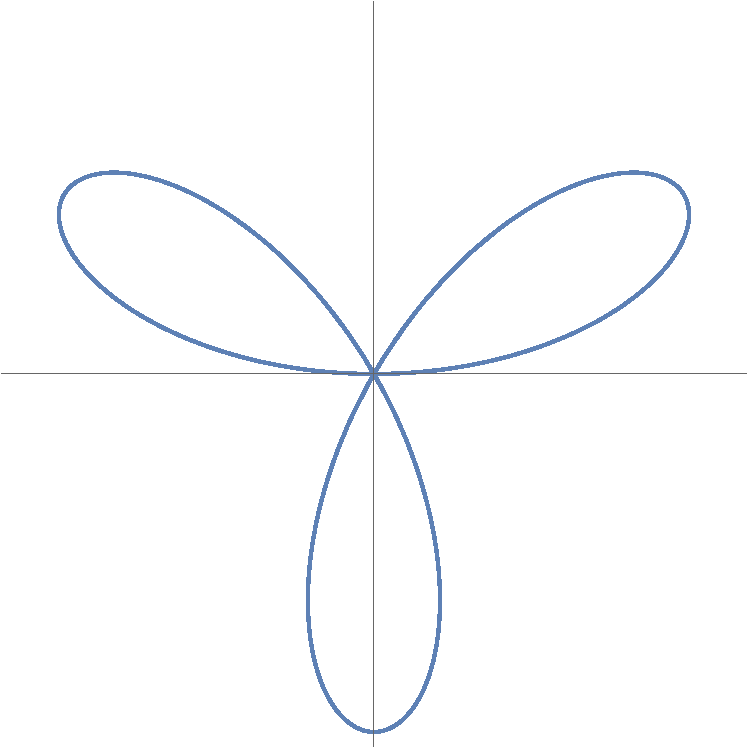
\includegraphics[trim={0 0 0 -4.5mm}, clip, height=1.7in]{6_Rose2} \newline \scriptsize{($C<0$ flips across $x$-axis) \newline $C$ petals} \vspace{3mm} &
		--- & 
		$\begin{array}{c}
		x=\sin({Ct})\cos{t}\\
		y=\sin({Ct})\sin{t},\\[8mm]
		\end{array}$ $0\leq t\leq 2\pi$ \newline $C$ odd \vspace{-14mm} & 
		$r(\theta)=\sin(C\theta)$ \newline \vspace{9mm} $C$ odd \vspace{-12mm} & \\
		
		\hline
		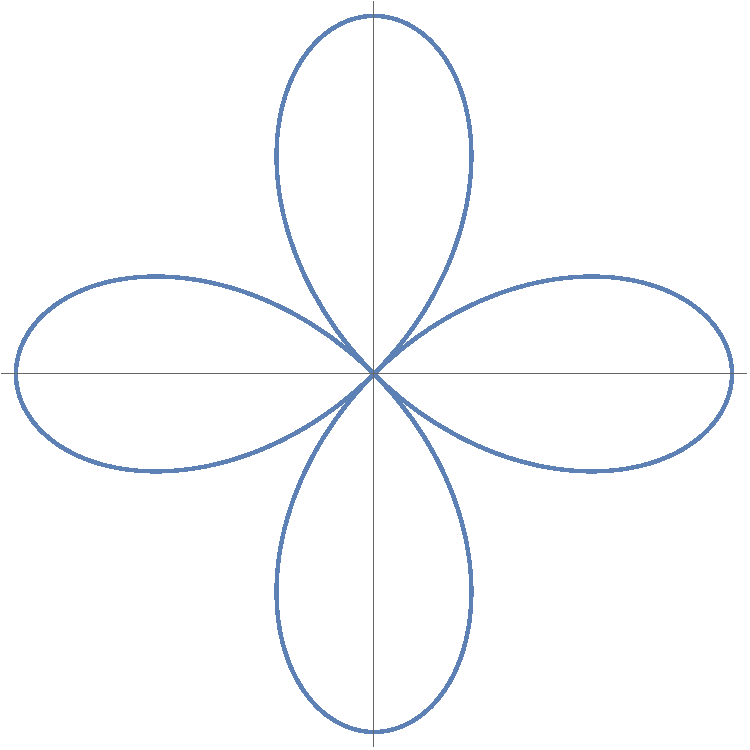
\includegraphics[trim={0 0 0 -4.5mm}, clip, height=1.7in]{6_Rose3} \newline \scriptsize{($C<0$ changes nothing) \newline $2C$ petals} \vspace{3mm} &
		--- & 
		$\begin{array}{c}
		x=\cos({Ct})\cos{t}\\
		y=\cos({Ct})\sin{t},\\[8mm]
		\end{array}$ $0\leq t\leq 2\pi$ \newline $C$ even \vspace{-14mm} & 
		$r(\theta)=\cos(C\theta)$ \newline \vspace{9mm} $C$ even \vspace{-12mm} & \\
		
		\hline
		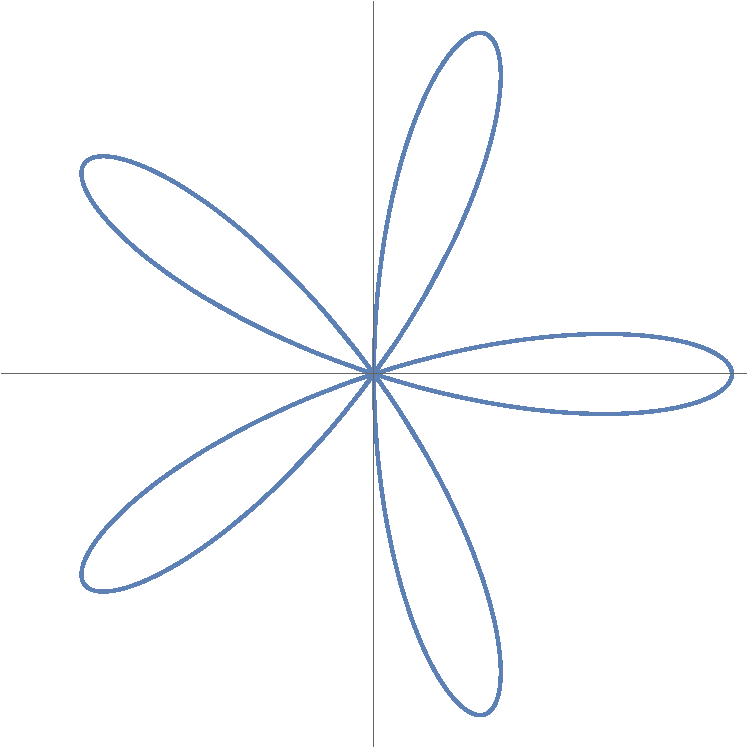
\includegraphics[trim={0 0 0 -4.5mm}, clip, height=1.7in]{6_Rose4} \newline \scriptsize{($C<0$ changes nothing) \newline $C$ petals} \vspace{3mm} &
		--- & 
		$\begin{array}{c}
		x=\cos({Ct})\cos{t}\\
		y=\cos({Ct})\sin{t},\\[8mm]
		\end{array}$ $0\leq t\leq 2\pi$ \newline $C$ odd \vspace{-14mm} & 
		$r(\theta)=\cos(C\theta)$ \newline \vspace{9mm} $C$ odd \vspace{-12mm} & \\
		
		\hline
	\end{tabular}
	\end{center}
\end{document}